% ******************************* Thesis Appendix A ****************************
\chapter{Signal Model Systematics}
\label{ch:app_sig_syst}

\section*{\texttt{T2cc}}
\label{sec:t2cc_syst_plots}

\newpage
\subsection*{Jet Energy Scale}
\label{sec:t2cc_jes_plots}

\begin{figure}[ht!]
  \centering
  \begin{subfigure}[b]{0.32\textwidth}
    \includegraphics[width=\textwidth, page=4]{Figs/sms/t2cc/v24/JES_T2cc_v24_eq0b_le3j_incl.pdf}
    \caption{\njlow, $\nb = 0$.}
  \end{subfigure}
  \begin{subfigure}[b]{0.32\textwidth}
    \includegraphics[width=\textwidth, page=5]{Figs/sms/t2cc/v24/JES_T2cc_v24_eq0b_le3j_incl.pdf}
    \caption{\njlow, $\nb = 0$.}
  \end{subfigure}
  \begin{subfigure}[b]{0.32\textwidth}
    \includegraphics[width=\textwidth, page=6]{Figs/sms/t2cc/v24/JES_T2cc_v24_eq0b_le3j_incl.pdf}
    \caption{\njlow, $\nb = 0$.}
    \label{fig:sms-jes-t2cc-le3j-0b}
  \end{subfigure}\\
  \begin{subfigure}[b]{0.32\textwidth}
    \includegraphics[width=\textwidth, page=4]{Figs/sms/t2cc/v24/JES_T2cc_v24_eq1b_le3j_incl.pdf}
    \caption{\njlow, $\nb = 1$.}
  \end{subfigure}
  \begin{subfigure}[b]{0.32\textwidth}
    \includegraphics[width=\textwidth, page=5]{Figs/sms/t2cc/v24/JES_T2cc_v24_eq1b_le3j_incl.pdf}
    \caption{\njlow, $\nb = 1$.}
  \end{subfigure}
  \begin{subfigure}[b]{0.32\textwidth}
    \includegraphics[width=\textwidth, page=6]{Figs/sms/t2cc/v24/JES_T2cc_v24_eq1b_le3j_incl.pdf}
    \caption{\njlow, $\nb = 1$.}
    \label{fig:sms-jes-t2cc-le3j-1b}
  \end{subfigure}\\
  \begin{subfigure}[b]{0.32\textwidth}
    \includegraphics[width=\textwidth, page=4]{Figs/sms/t2cc/v24/JES_T2cc_v24_eq0b_ge4j_incl.pdf}
    \caption{\njhigh, $\nb = 0$.}
  \end{subfigure}
  \begin{subfigure}[b]{0.32\textwidth}
    \includegraphics[width=\textwidth, page=5]{Figs/sms/t2cc/v24/JES_T2cc_v24_eq0b_ge4j_incl.pdf}
    \caption{\njhigh, $\nb = 0$.}
  \end{subfigure}
  \begin{subfigure}[b]{0.32\textwidth}
    \includegraphics[width=\textwidth, page=6]{Figs/sms/t2cc/v24/JES_T2cc_v24_eq0b_ge4j_incl.pdf}
    \caption{\njhigh, $\nb = 0$.}
    \label{fig:sms-jes-t2cc-ge4j-0b}
  \end{subfigure}\\
  \begin{subfigure}[b]{0.32\textwidth}
    \includegraphics[width=\textwidth, page=4]{Figs/sms/t2cc/v24/JES_T2cc_v24_eq1b_ge4j_incl.pdf}
    \caption{\njhigh, $\nb = 1$.}
  \end{subfigure}
  \begin{subfigure}[b]{0.32\textwidth}
    \includegraphics[width=\textwidth, page=5]{Figs/sms/t2cc/v24/JES_T2cc_v24_eq1b_ge4j_incl.pdf}
    \caption{\njhigh, $\nb = 1$.}
  \end{subfigure}
  \begin{subfigure}[b]{0.32\textwidth}
    \includegraphics[width=\textwidth, page=6]{Figs/sms/t2cc/v24/JES_T2cc_v24_eq1b_ge4j_incl.pdf}
    \caption{\njhigh, $\nb = 1$.}
    \label{fig:sms-jes-t2cc-ge4j-1b}
  \end{subfigure}\\
  \caption{The relative change in acceptance times signal efficiency for the
  \texttt{T2cc} model for downwards (left) and upwards (middle) fluctuations
  of all jet energies by the uncertainty of the jet energy scale, and the 
  derived systematic values (right). Each set of plots corresponds to one of
  the four most sensitive analysis categories (\nb, \nj), with the inclusive 
  requirement \HT>200 \gev.}
  \label{fig:sms-jes-t2cc}
\end{figure}


\newpage
\subsection*{PDF}
\label{sec:t2cc_pdf_plots}
\emph{FIND PLOTS}

% \begin{figure}[ht!]
%   \centering
%   \begin{subfigure}[b]{0.6\textwidth}
%     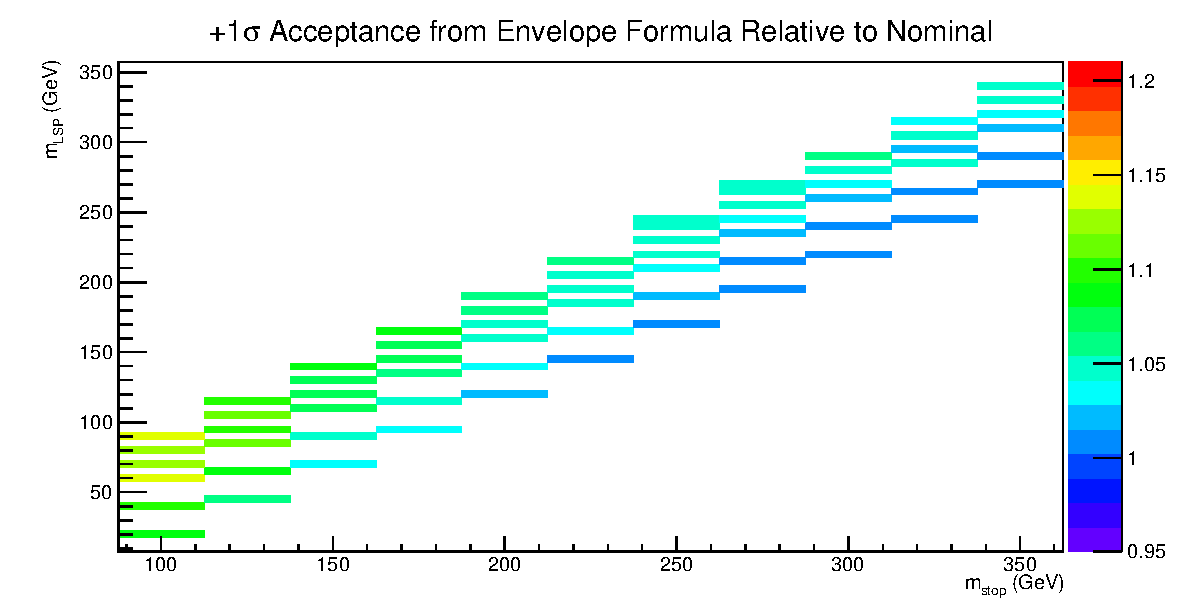
\includegraphics[width=\textwidth]{Figs/sms/t2cc/acc_pSigmaRel_m0_m12}
%     \caption{$+1\sigma$}
%     \label{fig:sms-pdf-up-t2cc}
%   \end{subfigure}
%   \begin{subfigure}[b]{0.6\textwidth}
%     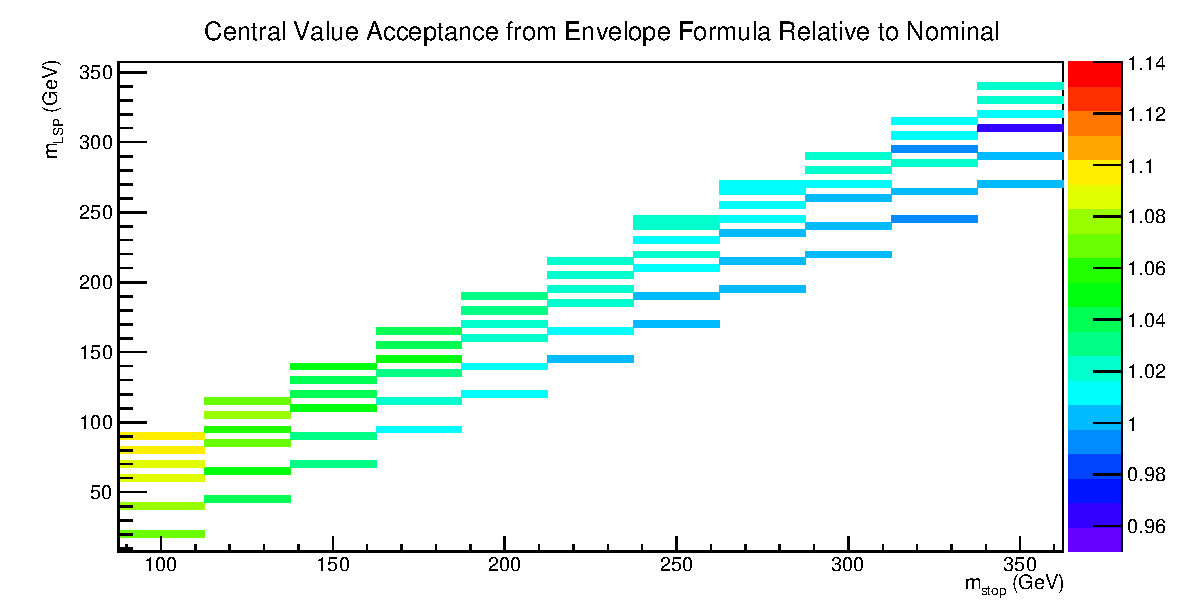
\includegraphics[width=\textwidth]{Figs/sms/t2cc/acc_cvRel_m0_m12}
%     \caption{Nominal}
%     \label{fig:sms-pdf-nominal-t2cc}
%   \end{subfigure}
%   \begin{subfigure}[b]{0.6\textwidth}
%     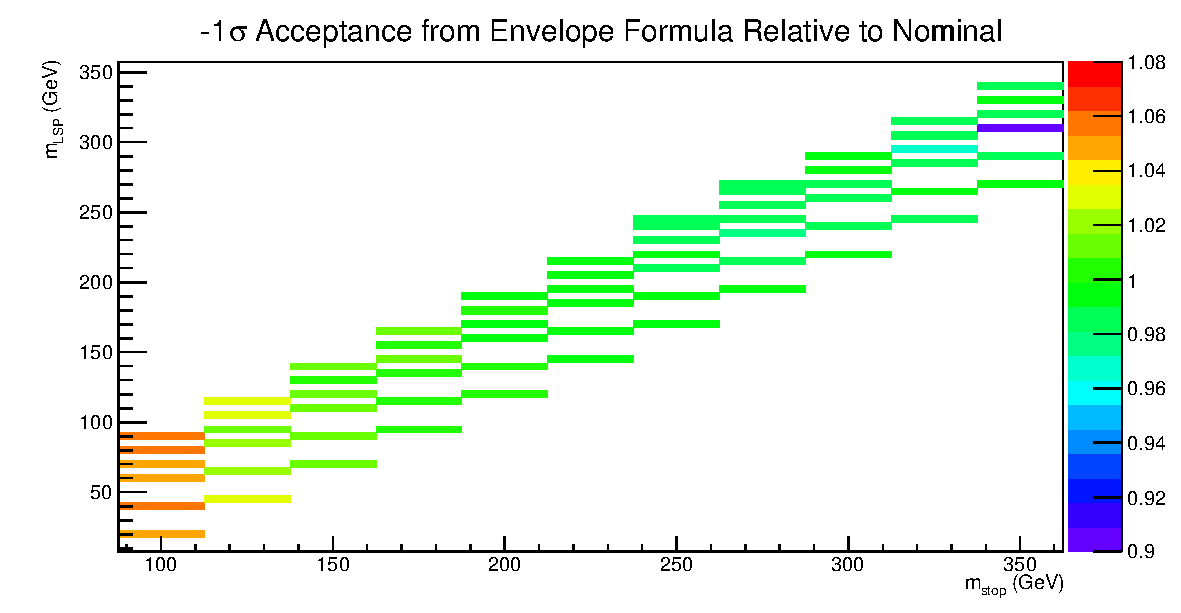
\includegraphics[width=\textwidth]{Figs/sms/t2cc/acc_mSigmaRel_m0_m12}
%     \caption{$-1\sigma$}
%     \label{fig:sms-pdf-down-t2cc}
%   \end{subfigure}
%   \caption{PDF shit yo}
%   \label{fig:sms-pdf-t2cc}
% \end{figure}


\newpage
\subsection*{Initial State Radiation}
\label{sec:t2cc_isr_plots}

\begin{figure}[ht!]
  \centering
  \begin{subfigure}[b]{0.32\textwidth}
    \includegraphics[width=\textwidth, page=4]{Figs/sms/t2cc/v24/ISR_T2cc_v24_eq0b_le3j_incl.pdf}
    \caption{\njlow, $\nb = 0$.}
  \end{subfigure}
  \begin{subfigure}[b]{0.32\textwidth}
    \includegraphics[width=\textwidth, page=5]{Figs/sms/t2cc/v24/ISR_T2cc_v24_eq0b_le3j_incl.pdf}
    \caption{\njlow, $\nb = 0$.}
  \end{subfigure}
  \begin{subfigure}[b]{0.32\textwidth}
    \includegraphics[width=\textwidth, page=6]{Figs/sms/t2cc/v24/ISR_T2cc_v24_eq0b_le3j_incl.pdf}
    \caption{\njlow, $\nb = 0$.}
  \end{subfigure}\\
  \begin{subfigure}[b]{0.32\textwidth}
    \includegraphics[width=\textwidth, page=4]{Figs/sms/t2cc/v24/ISR_T2cc_v24_eq1b_le3j_incl.pdf}
    \caption{\njlow, $\nb = 1$.}
  \end{subfigure}
  \begin{subfigure}[b]{0.32\textwidth}
    \includegraphics[width=\textwidth, page=5]{Figs/sms/t2cc/v24/ISR_T2cc_v24_eq1b_le3j_incl.pdf}
    \caption{\njlow, $\nb = 1$.}
  \end{subfigure}
  \begin{subfigure}[b]{0.32\textwidth}
    \includegraphics[width=\textwidth, page=6]{Figs/sms/t2cc/v24/ISR_T2cc_v24_eq1b_le3j_incl.pdf}
    \caption{\njlow, $\nb = 1$.}
  \end{subfigure}\\
  \begin{subfigure}[b]{0.32\textwidth}
    \includegraphics[width=\textwidth, page=4]{Figs/sms/t2cc/v24/ISR_T2cc_v24_eq0b_ge4j_incl.pdf}
    \caption{\njhigh, $\nb = 0$.}
  \end{subfigure}
  \begin{subfigure}[b]{0.32\textwidth}
    \includegraphics[width=\textwidth, page=5]{Figs/sms/t2cc/v24/ISR_T2cc_v24_eq0b_ge4j_incl.pdf}
    \caption{\njhigh, $\nb = 0$.}
  \end{subfigure}
  \begin{subfigure}[b]{0.32\textwidth}
    \includegraphics[width=\textwidth, page=6]{Figs/sms/t2cc/v24/ISR_T2cc_v24_eq0b_ge4j_incl.pdf}
    \caption{\njhigh, $\nb = 0$.}
  \end{subfigure}\\
  \begin{subfigure}[b]{0.32\textwidth}
    \includegraphics[width=\textwidth, page=4]{Figs/sms/t2cc/v24/ISR_T2cc_v24_eq1b_ge4j_incl.pdf}
    \caption{\njhigh, $\nb = 1$.}
  \end{subfigure}
  \begin{subfigure}[b]{0.32\textwidth}
    \includegraphics[width=\textwidth, page=5]{Figs/sms/t2cc/v24/ISR_T2cc_v24_eq1b_ge4j_incl.pdf}
    \caption{\njhigh, $\nb = 1$.}
  \end{subfigure}
  \begin{subfigure}[b]{0.32\textwidth}
    \includegraphics[width=\textwidth, page=6]{Figs/sms/t2cc/v24/ISR_T2cc_v24_eq1b_ge4j_incl.pdf}
    \caption{\njhigh, $\nb = 1$.}
  \end{subfigure}\\
  \caption{The relative change in acceptance times signal efficiency for the
  \texttt{T2cc} model for downwards (left) and upwards (middle) fluctuations
  of the global event weight equal to the magnitude of the ISR corrections,
  and the derived systematic values (right). Each set of plots corresponds
  to one of the four most sensitive analysis categories (\nb, \nj), with the
  inclusive requirement \HT>200 \gev.}
  \label{fig:sms-isr-t2cc}
\end{figure}


\newpage
\subsection*{B-tag Scale Factor}
\label{sec:t2cc_btag_plots}

\begin{figure}[ht!]
  \centering
  \begin{subfigure}[b]{0.32\textwidth}
    \includegraphics[width=\textwidth, page=4]{Figs/sms/t2cc/v24/bTag_T2cc_v24_eq0b_le3j_incl.pdf}
    \caption{\njlow, $\nb = 0$.}
  \end{subfigure}
  \begin{subfigure}[b]{0.32\textwidth}
    \includegraphics[width=\textwidth, page=5]{Figs/sms/t2cc/v24/bTag_T2cc_v24_eq0b_le3j_incl.pdf}
    \caption{\njlow, $\nb = 0$.}
  \end{subfigure}
  \begin{subfigure}[b]{0.32\textwidth}
    \includegraphics[width=\textwidth, page=6]{Figs/sms/t2cc/v24/bTag_T2cc_v24_eq0b_le3j_incl.pdf}
    \caption{\njlow, $\nb = 0$.}
  \end{subfigure}\\
  \begin{subfigure}[b]{0.32\textwidth}
    \includegraphics[width=\textwidth, page=4]{Figs/sms/t2cc/v24/bTag_T2cc_v24_eq1b_le3j_incl.pdf}
    \caption{\njlow, $\nb = 1$.}
  \end{subfigure}
  \begin{subfigure}[b]{0.32\textwidth}
    \includegraphics[width=\textwidth, page=5]{Figs/sms/t2cc/v24/bTag_T2cc_v24_eq1b_le3j_incl.pdf}
    \caption{\njlow, $\nb = 1$.}
  \end{subfigure}
  \begin{subfigure}[b]{0.32\textwidth}
    \includegraphics[width=\textwidth, page=6]{Figs/sms/t2cc/v24/bTag_T2cc_v24_eq1b_le3j_incl.pdf}
    \caption{\njlow, $\nb = 1$.}
    \label{fig:sms-btag-t2cc-le3j-1b}
  \end{subfigure}\\
  \begin{subfigure}[b]{0.32\textwidth}
    \includegraphics[width=\textwidth, page=4]{Figs/sms/t2cc/v24/bTag_T2cc_v24_eq0b_ge4j_incl.pdf}
    \caption{\njhigh, $\nb = 0$.}
  \end{subfigure}
  \begin{subfigure}[b]{0.32\textwidth}
    \includegraphics[width=\textwidth, page=5]{Figs/sms/t2cc/v24/bTag_T2cc_v24_eq0b_ge4j_incl.pdf}
    \caption{\njhigh, $\nb = 0$.}
  \end{subfigure}
  \begin{subfigure}[b]{0.32\textwidth}
    \includegraphics[width=\textwidth, page=6]{Figs/sms/t2cc/v24/bTag_T2cc_v24_eq0b_ge4j_incl.pdf}
    \caption{\njhigh, $\nb = 0$.}
  \end{subfigure}\\
  \begin{subfigure}[b]{0.32\textwidth}
    \includegraphics[width=\textwidth, page=4]{Figs/sms/t2cc/v24/bTag_T2cc_v24_eq1b_ge4j_incl.pdf}
    \caption{\njhigh, $\nb = 1$.}
  \end{subfigure}
  \begin{subfigure}[b]{0.32\textwidth}
    \includegraphics[width=\textwidth, page=5]{Figs/sms/t2cc/v24/bTag_T2cc_v24_eq1b_ge4j_incl.pdf}
    \caption{\njhigh, $\nb = 1$.}
  \end{subfigure}
  \begin{subfigure}[b]{0.32\textwidth}
    \includegraphics[width=\textwidth, page=6]{Figs/sms/t2cc/v24/bTag_T2cc_v24_eq1b_ge4j_incl.pdf}
    \caption{\njhigh, $\nb = 1$.}
  \end{subfigure}\\
  \caption{The relative change in acceptance times signal efficiency for the
  \texttt{T2cc} model for downwards (left) and upwards (middle) fluctuations
  of global event weight according to the uncertainties of the Btag scale 
  factors,
  and the derived systematic values (right). Each set of plots corresponds
  to one of the four most sensitive analysis categories (\nb, \nj), with the
  inclusive requirement \HT>200 \gev.}
  \label{fig:sms-btag-t2cc}
\end{figure}


\newpage
\subsection*{\mhtmet cut}
\label{sec:t2cc_mhtmet_plots}

\begin{figure}[h!]
  \centering
  \begin{subfigure}[b]{0.4\textwidth}
    \includegraphics[width=\textwidth, page=3]{Figs/sms/t2cc/v24/MHT_MET_T2cc_v24_eq0b_le3j_incl.pdf}
    \caption{\njlow, $\nb = 0$.}
  \end{subfigure}
  \begin{subfigure}[b]{0.4\textwidth}
    \includegraphics[width=\textwidth, page=3]{Figs/sms/t2cc/v24/MHT_MET_T2cc_v24_eq1b_le3j_incl.pdf}
    \caption{\njlow, $\nb = 1$.}
  \end{subfigure}\\
  \begin{subfigure}[b]{0.4\textwidth}
    \includegraphics[width=\textwidth, page=3]{Figs/sms/t2cc/v24/MHT_MET_T2cc_v24_eq0b_ge4j_incl.pdf}
    \caption{\njhigh, $\nb = 0$.}
  \end{subfigure}
  \begin{subfigure}[b]{0.4\textwidth}
    \includegraphics[width=\textwidth, page=3]{Figs/sms/t2cc/v24/MHT_MET_T2cc_v24_eq1b_ge4j_incl.pdf}
    \caption{\njhigh, $\nb = 1$.}
  \end{subfigure}\\
  \caption{The acceptance of the \mhtmet cut as a function of the \texttt{T2cc}
  mass plane. Each plot represents one of the four most sensitive 
  analysis cateogires (\nb, \nj), with the inclusive requirement \HT>200 \gev.}
  \label{fig:sms-mhtmet-t2cc}
\end{figure}


\newpage
\subsection*{Dead ECAL cut}
\label{sec:t2cc_deadecal_plots}

\begin{figure}[h!]
  \centering
  \begin{subfigure}[b]{0.4\textwidth}
    \includegraphics[width=\textwidth, page=3]{Figs/sms/t2cc/v24/DeadECAL_T2cc_v24_eq0b_le3j_incl.pdf}
    \caption{\njlow, $\nb = 0$.}
  \end{subfigure}
  \begin{subfigure}[b]{0.4\textwidth}
    \includegraphics[width=\textwidth, page=3]{Figs/sms/t2cc/v24/DeadECAL_T2cc_v24_eq1b_le3j_incl.pdf}
    \caption{\njlow, $\nb = 1$.}
  \end{subfigure}\\
  \begin{subfigure}[b]{0.4\textwidth}
    \includegraphics[width=\textwidth, page=3]{Figs/sms/t2cc/v24/DeadECAL_T2cc_v24_eq0b_ge4j_incl.pdf}
    \caption{\njhigh, $\nb = 0$.}
  \end{subfigure}
  \begin{subfigure}[b]{0.4\textwidth}
    \includegraphics[width=\textwidth, page=3]{Figs/sms/t2cc/v24/DeadECAL_T2cc_v24_eq1b_ge4j_incl.pdf}
    \caption{\njhigh, $\nb = 1$.}
  \end{subfigure}\\
  \caption{The acceptance of the DeadECAL cut as a function of the \texttt{T2cc}
  mass plane. Each plot represents one of the four most sensitive 
  analysis cateogires (\nb, \nj), with the inclusive requirement \HT>200 \gev.}
  \label{fig:sms-deadecal-t2cc}
\end{figure}


\newpage
\section*{\texttt{T2degen}}
\label{sec:t2degen_syst_plots}

\newpage
\subsection*{Jet Energy Scale}
\label{sec:t2degen_jes_plots}

\begin{figure}[ht!]
  \centering
  \begin{subfigure}[b]{0.32\textwidth}
    \includegraphics[width=\textwidth, page=4]{Figs/sms/t2degen/v5/JES_T2_4body_v5_eq0b_le3j_incl.pdf}
    \caption{\njlow, $\nb = 0$.}
  \end{subfigure}
  \begin{subfigure}[b]{0.32\textwidth}
    \includegraphics[width=\textwidth, page=5]{Figs/sms/t2degen/v5/JES_T2_4body_v5_eq0b_le3j_incl.pdf}
    \caption{\njlow, $\nb = 0$.}
  \end{subfigure}
  \begin{subfigure}[b]{0.32\textwidth}
    \includegraphics[width=\textwidth, page=6]{Figs/sms/t2degen/v5/JES_T2_4body_v5_eq0b_le3j_incl.pdf}
    \caption{\njlow, $\nb = 0$.}
    \label{fig:sms-jes-tdegen-le3j-0b}
  \end{subfigure}\\
  \begin{subfigure}[b]{0.32\textwidth}
    \includegraphics[width=\textwidth, page=4]{Figs/sms/t2degen/v5/JES_T2_4body_v5_eq1b_le3j_incl.pdf}
    \caption{\njlow, $\nb = 1$.}
  \end{subfigure}
  \begin{subfigure}[b]{0.32\textwidth}
    \includegraphics[width=\textwidth, page=5]{Figs/sms/t2degen/v5/JES_T2_4body_v5_eq1b_le3j_incl.pdf}
    \caption{\njlow, $\nb = 1$.}
  \end{subfigure}
  \begin{subfigure}[b]{0.32\textwidth}
    \includegraphics[width=\textwidth, page=6]{Figs/sms/t2degen/v5/JES_T2_4body_v5_eq1b_le3j_incl.pdf}
    \caption{\njlow, $\nb = 1$.}
    \label{fig:sms-jes-tdegen-le3j-1b}
  \end{subfigure}\\
  \begin{subfigure}[b]{0.32\textwidth}
    \includegraphics[width=\textwidth, page=4]{Figs/sms/t2degen/v5/JES_T2_4body_v5_eq0b_ge4j_incl.pdf}
    \caption{\njhigh, $\nb = 0$.}
  \end{subfigure}
  \begin{subfigure}[b]{0.32\textwidth}
    \includegraphics[width=\textwidth, page=5]{Figs/sms/t2degen/v5/JES_T2_4body_v5_eq0b_ge4j_incl.pdf}
    \caption{\njhigh, $\nb = 0$.}
  \end{subfigure}
  \begin{subfigure}[b]{0.32\textwidth}
    \includegraphics[width=\textwidth, page=6]{Figs/sms/t2degen/v5/JES_T2_4body_v5_eq0b_ge4j_incl.pdf}
    \caption{\njhigh, $\nb = 0$.}
    \label{fig:sms-jes-tdegen-ge4j-0b}
  \end{subfigure}\\
  \begin{subfigure}[b]{0.32\textwidth}
    \includegraphics[width=\textwidth, page=4]{Figs/sms/t2degen/v5/JES_T2_4body_v5_eq1b_ge4j_incl.pdf}
    \caption{\njhigh, $\nb = 1$.}
  \end{subfigure}
  \begin{subfigure}[b]{0.32\textwidth}
    \includegraphics[width=\textwidth, page=5]{Figs/sms/t2degen/v5/JES_T2_4body_v5_eq1b_ge4j_incl.pdf}
    \caption{\njhigh, $\nb = 1$.}
  \end{subfigure}
  \begin{subfigure}[b]{0.32\textwidth}
    \includegraphics[width=\textwidth, page=6]{Figs/sms/t2degen/v5/JES_T2_4body_v5_eq1b_ge4j_incl.pdf}
    \caption{\njhigh, $\nb = 1$.}
    \label{fig:sms-jes-tdegen-ge4j-1b}
  \end{subfigure}\\
  \caption{The relative change in acceptance times signal efficiency for the
  \texttt{T2Degen} model for downwards (left) and upwards (middle) fluctuations
  of all jet energies by the uncertainty of the jet energy scale, and the 
  derived systematic values (right). Each set of plots corresponds to one of
  the four most sensitive analysis categories (\nb, \nj), with the inclusive 
  requirement \HT>200 \gev.}
  \label{fig:sms-jes-t2degen}
\end{figure}


\newpage
\subsection*{PDF}
\label{sec:t2degen_pdf_plots}
\emph{FIND PLOTS}

% \begin{figure}[ht!]
%   \centering
%   \begin{subfigure}[b]{0.6\textwidth}
%     \includegraphics[width=\textwidth]{Figs/sms/t2cc/acc_pSigmaRel_m0_m12}
%     \caption{$+1\sigma$}
%     \label{fig:sms-pdf-up-t2degen}
%   \end{subfigure}
%   \begin{subfigure}[b]{0.6\textwidth}
%     \includegraphics[width=\textwidth]{Figs/sms/t2cc/acc_cvRel_m0_m12}
%     \caption{Nominal}
%     \label{fig:sms-pdf-nominal-t2degen}
%   \end{subfigure}
%   \begin{subfigure}[b]{0.6\textwidth}
%     \includegraphics[width=\textwidth]{Figs/sms/t2cc/acc_mSigmaRel_m0_m12}
%     \caption{$-1\sigma$}
%     \label{fig:sms-pdf-down-t2degen}
%   \end{subfigure}
%   \caption{PDF shit yo}
%   \label{fig:sms-pdf-t2degen}
% \end{figure}


\newpage
\subsection*{Initial State Radiation}
\label{sec:t2degen_isr_plots}

\begin{figure}[ht!]
  \centering
  \begin{subfigure}[b]{0.32\textwidth}
    \includegraphics[width=\textwidth, page=4]{Figs/sms/t2degen/v5/ISR_T2_4body_v5_eq0b_le3j_incl.pdf}
    \caption{\njlow, $\nb = 0$.}
  \end{subfigure}
  \begin{subfigure}[b]{0.32\textwidth}
    \includegraphics[width=\textwidth, page=5]{Figs/sms/t2degen/v5/ISR_T2_4body_v5_eq0b_le3j_incl.pdf}
    \caption{\njlow, $\nb = 0$.}
  \end{subfigure}
  \begin{subfigure}[b]{0.32\textwidth}
    \includegraphics[width=\textwidth, page=6]{Figs/sms/t2degen/v5/ISR_T2_4body_v5_eq0b_le3j_incl.pdf}
    \caption{\njlow, $\nb = 0$.}
  \end{subfigure}\\
  \begin{subfigure}[b]{0.32\textwidth}
    \includegraphics[width=\textwidth, page=4]{Figs/sms/t2degen/v5/ISR_T2_4body_v5_eq1b_le3j_incl.pdf}
    \caption{\njlow, $\nb = 1$.}
  \end{subfigure}
  \begin{subfigure}[b]{0.32\textwidth}
    \includegraphics[width=\textwidth, page=5]{Figs/sms/t2degen/v5/ISR_T2_4body_v5_eq1b_le3j_incl.pdf}
    \caption{\njlow, $\nb = 1$.}
  \end{subfigure}
  \begin{subfigure}[b]{0.32\textwidth}
    \includegraphics[width=\textwidth, page=6]{Figs/sms/t2degen/v5/ISR_T2_4body_v5_eq1b_le3j_incl.pdf}
    \caption{\njlow, $\nb = 1$.}
  \end{subfigure}\\
  \begin{subfigure}[b]{0.32\textwidth}
    \includegraphics[width=\textwidth, page=4]{Figs/sms/t2degen/v5/ISR_T2_4body_v5_eq0b_ge4j_incl.pdf}
    \caption{\njhigh, $\nb = 0$.}
  \end{subfigure}
  \begin{subfigure}[b]{0.32\textwidth}
    \includegraphics[width=\textwidth, page=5]{Figs/sms/t2degen/v5/ISR_T2_4body_v5_eq0b_ge4j_incl.pdf}
    \caption{\njhigh, $\nb = 0$.}
  \end{subfigure}
  \begin{subfigure}[b]{0.32\textwidth}
    \includegraphics[width=\textwidth, page=6]{Figs/sms/t2degen/v5/ISR_T2_4body_v5_eq0b_ge4j_incl.pdf}
    \caption{\njhigh, $\nb = 0$.}
  \end{subfigure}\\
  \begin{subfigure}[b]{0.32\textwidth}
    \includegraphics[width=\textwidth, page=4]{Figs/sms/t2degen/v5/ISR_T2_4body_v5_eq1b_ge4j_incl.pdf}
    \caption{\njhigh, $\nb = 1$.}
  \end{subfigure}
  \begin{subfigure}[b]{0.32\textwidth}
    \includegraphics[width=\textwidth, page=5]{Figs/sms/t2degen/v5/ISR_T2_4body_v5_eq1b_ge4j_incl.pdf}
    \caption{\njhigh, $\nb = 1$.}
  \end{subfigure}
  \begin{subfigure}[b]{0.32\textwidth}
    \includegraphics[width=\textwidth, page=6]{Figs/sms/t2degen/v5/ISR_T2_4body_v5_eq1b_ge4j_incl.pdf}
    \caption{\njhigh, $\nb = 1$.}
  \end{subfigure}\\
  \caption{The relative change in acceptance times signal efficiency for the
  \texttt{T2Degen} model for downwards (left) and upwards (middle) fluctuations
  of the global event weight equal to the magnitude of the ISR corrections,
  and the derived systematic values (right). Each set of plots corresponds
  to one of the four most sensitive analysis categories (\nb, \nj), with the
  inclusive requirement \HT>200 \gev.}
  \label{fig:sms-isr-t2degen}
\end{figure}


\newpage
\subsection*{B-tag Scale Factor}
\label{sec:t2degen_btag_plots}

\begin{figure}[ht!]
  \centering
  \begin{subfigure}[b]{0.32\textwidth}
    \includegraphics[width=\textwidth, page=4]{Figs/sms/t2degen/v5/bTag_T2_4body_v5_eq0b_le3j_incl.pdf}
    \caption{\njlow, $\nb = 0$.}
  \end{subfigure}
  \begin{subfigure}[b]{0.32\textwidth}
    \includegraphics[width=\textwidth, page=5]{Figs/sms/t2degen/v5/bTag_T2_4body_v5_eq0b_le3j_incl.pdf}
    \caption{\njlow, $\nb = 0$.}
  \end{subfigure}
  \begin{subfigure}[b]{0.32\textwidth}
    \includegraphics[width=\textwidth, page=6]{Figs/sms/t2degen/v5/bTag_T2_4body_v5_eq0b_le3j_incl.pdf}
    \caption{\njlow, $\nb = 0$.}
  \end{subfigure}\\
  \begin{subfigure}[b]{0.32\textwidth}
    \includegraphics[width=\textwidth, page=4]{Figs/sms/t2degen/v5/bTag_T2_4body_v5_eq1b_le3j_incl.pdf}
    \caption{\njlow, $\nb = 1$.}
  \end{subfigure}
  \begin{subfigure}[b]{0.32\textwidth}
    \includegraphics[width=\textwidth, page=5]{Figs/sms/t2degen/v5/bTag_T2_4body_v5_eq1b_le3j_incl.pdf}
    \caption{\njlow, $\nb = 1$.}
  \end{subfigure}
  \begin{subfigure}[b]{0.32\textwidth}
    \includegraphics[width=\textwidth, page=6]{Figs/sms/t2degen/v5/bTag_T2_4body_v5_eq1b_le3j_incl.pdf}
    \caption{\njlow, $\nb = 1$.}
  \end{subfigure}\\
  \begin{subfigure}[b]{0.32\textwidth}
    \includegraphics[width=\textwidth, page=4]{Figs/sms/t2degen/v5/bTag_T2_4body_v5_eq0b_ge4j_incl.pdf}
    \caption{\njhigh, $\nb = 0$.}
  \end{subfigure}
  \begin{subfigure}[b]{0.32\textwidth}
    \includegraphics[width=\textwidth, page=5]{Figs/sms/t2degen/v5/bTag_T2_4body_v5_eq0b_ge4j_incl.pdf}
    \caption{\njhigh, $\nb = 0$.}
  \end{subfigure}
  \begin{subfigure}[b]{0.32\textwidth}
    \includegraphics[width=\textwidth, page=6]{Figs/sms/t2degen/v5/bTag_T2_4body_v5_eq0b_ge4j_incl.pdf}
    \caption{\njhigh, $\nb = 0$.}
  \end{subfigure}\\
  \begin{subfigure}[b]{0.32\textwidth}
    \includegraphics[width=\textwidth, page=4]{Figs/sms/t2degen/v5/bTag_T2_4body_v5_eq1b_ge4j_incl.pdf}
    \caption{\njhigh, $\nb = 1$.}
  \end{subfigure}
  \begin{subfigure}[b]{0.32\textwidth}
    \includegraphics[width=\textwidth, page=5]{Figs/sms/t2degen/v5/bTag_T2_4body_v5_eq1b_ge4j_incl.pdf}
    \caption{\njhigh, $\nb = 1$.}
  \end{subfigure}
  \begin{subfigure}[b]{0.32\textwidth}
    \includegraphics[width=\textwidth, page=6]{Figs/sms/t2degen/v5/bTag_T2_4body_v5_eq1b_ge4j_incl.pdf}
    \caption{\njhigh, $\nb = 1$.}
  \end{subfigure}\\
  \caption{The relative change in acceptance times signal efficiency for the
  \texttt{T2Degen} model for downwards (left) and upwards (middle) fluctuations
  of global event weight according to the uncertainties of the Btag scale 
  factors,
  and the derived systematic values (right). Each set of plots corresponds
  to one of the four most sensitive analysis categories (\nb, \nj), with the
  inclusive requirement \HT>200 \gev.}
  \label{fig:sms-btag-t2degen}
\end{figure}


\newpage
\subsection*{\mhtmet cut}
\label{sec:t2degen_mhtmet_plots}

\begin{figure}[h!]
  \centering
  \begin{subfigure}[b]{0.4\textwidth}
    \includegraphics[width=\textwidth, page=3]{Figs/sms/t2degen/v5/MHT_MET_T2_4body_v5_eq0b_le3j_incl.pdf}
    \caption{\njlow, $\nb = 0$.}
  \end{subfigure}
  \begin{subfigure}[b]{0.4\textwidth}
    \includegraphics[width=\textwidth, page=3]{Figs/sms/t2degen/v5/MHT_MET_T2_4body_v5_eq1b_le3j_incl.pdf}
    \caption{\njlow, $\nb = 1$.}
  \end{subfigure}\\
  \begin{subfigure}[b]{0.4\textwidth}
    \includegraphics[width=\textwidth, page=3]{Figs/sms/t2degen/v5/MHT_MET_T2_4body_v5_eq0b_ge4j_incl.pdf}
    \caption{\njhigh, $\nb = 0$.}
  \end{subfigure}
  \begin{subfigure}[b]{0.4\textwidth}
    \includegraphics[width=\textwidth, page=3]{Figs/sms/t2degen/v5/MHT_MET_T2_4body_v5_eq1b_ge4j_incl.pdf}
    \caption{\njhigh, $\nb = 1$.}
  \end{subfigure}\\
  \caption{The acceptance of the \mhtmet cut as a function of the \texttt{T2degen}
  mass plane. Each plot represents one of the four most sensitive 
  analysis cateogires (\nb, \nj), with the inclusive requirement \HT>200 \gev.}
  \label{fig:sms-mhtmet-t2degen}
\end{figure}


\newpage
\subsection*{Dead ECAL cut}
\label{sec:t2degen_deadecal_plots}

\begin{figure}[h!]
  \centering
  \begin{subfigure}[b]{0.4\textwidth}
    \includegraphics[width=\textwidth, page=3]{Figs/sms/t2degen/v5/DeadECAL_T2_4body_v5_eq0b_le3j_incl.pdf}
    \caption{\njlow, $\nb = 0$.}
  \end{subfigure}
  \begin{subfigure}[b]{0.4\textwidth}
    \includegraphics[width=\textwidth, page=3]{Figs/sms/t2degen/v5/DeadECAL_T2_4body_v5_eq1b_le3j_incl.pdf}
    \caption{\njlow, $\nb = 1$.}
  \end{subfigure}\\
  \begin{subfigure}[b]{0.4\textwidth}
    \includegraphics[width=\textwidth, page=3]{Figs/sms/t2degen/v5/DeadECAL_T2_4body_v5_eq0b_ge4j_incl.pdf}
    \caption{\njhigh, $\nb = 0$.}
  \end{subfigure}
  \begin{subfigure}[b]{0.4\textwidth}
    \includegraphics[width=\textwidth, page=3]{Figs/sms/t2degen/v5/DeadECAL_T2_4body_v5_eq1b_ge4j_incl.pdf}
    \caption{\njhigh, $\nb = 1$.}
  \end{subfigure}\\
  \caption{The acceptance of the DeadECAL cut as a function of the \texttt{T2Degen}
  mass plane. Each plot represents one of the four most sensitive 
  analysis cateogires (\nb, \nj), with the inclusive requirement \HT>200 \gev.}
  \label{fig:sms-deadecal-t2degen}
\end{figure}
